\chapter{Μεθοδολογία}
\label{ch:methodology}

\section{Υπολογισμοί Απόστασης Στοιχειωδών Γεωμετρικών Αντικειμένων}
\subsection{Ευκλείδεια Απόσταση δύο Τριγώνων}
\label{subsec:tria_distance}
% Έστω τα τρίγωνα $P$ και $Q$ στον $\mathbb{R}^3$.
% Η Ευκλείδεια απόσταση $d(P,Q)$ μεταξύ των τριγώνων $P$ και $Q$
% ορίζεται ως:
% \[ d(P,Q) = \min_{p \in P, q \in Q} |p - q| \]
% όπου με $|p-q|$ συμβολίζεται η Ευκλείδεια απόσταση των σημείων 
% $p$ και $q$.

% Έστω p,q

\subsubsection{Ευκλείδεια Απόσταση δύο Ευθυγράμμων Τμημάτων}
\subsubsection{Ευκλείδεια Απόσταση Σημείου και Τριγώνου}
\subsection{Ευκλείδεια Απόσταση δύο \tl{AABB}}
Έστω τα ευθυγραμμισμένα με τους άξονες πλαίσια
$P$ και $Q$ στον $\mathbb{R}^3$.
Η Ευκλείδεια απόσταση $d(P,Q)$ μεταξύ των πλαισίων $P$ και $Q$
ορίζεται ως:
\[ d(P,Q) = \min_{p \in P, q \in Q} \lVert p - q \rVert \]
όπου με $\lVert p - q \rVert$ συμβολίζεται η Ευκλείδεια 
απόσταση των σημείων $p$ και $q$.

Ένα \tl{AABB} αναπαριστάται στη μνήμη από τα άκρα της κύριας 
διαγωνίου του.
Δηλαδή το σημείο $S$ με τις μικρότερες $x$, $y$, $z$ συντεταγμένες
και το σημείο $T$ με τις μεγαλύτερες $x$, $y$, $z$ συντεταγμένες.

\begin{figure}[h]
    \centering
    
    \newcommand{\Depth}{2}
    \newcommand{\Height}{2}
    \newcommand{\Width}{3}
    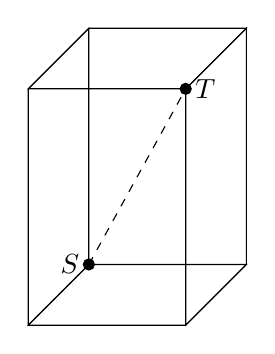
\begin{tikzpicture}
        \coordinate (O) at (0,0,0);
        \coordinate (A) at (0,\Width,0);
        \coordinate (B) at (0,\Width,\Height);
        \coordinate (C) at (0,0,\Height);
        \coordinate (D) at (\Depth,0,0);
        \coordinate (E) at (\Depth,\Width,0);
        \coordinate (F) at (\Depth,\Width,\Height);
        \coordinate (G) at (\Depth,0,\Height);

        \draw[] (O) -- (C) -- (G) -- (D) -- cycle;% Bottom Face
        \draw[] (O) -- (A) -- (E) -- (D) -- cycle;% Back Face
        \draw[] (O) -- (A) -- (B) -- (C) -- cycle;% Left Face
        \draw[] (D) -- (E) -- (F) -- (G) -- cycle;% Right Face
        \draw[] (C) -- (B) -- (F) -- (G) -- cycle;% Front Face
        \draw[] (A) -- (B) -- (F) -- (E) -- cycle;% Top Face

        \draw[fill=black] (O) circle (2pt) node[left]{$S$};
        \draw[fill=black] (F) circle (2pt) node[right]{$T$};
        \draw[dashed] (O) -- (F);
    \end{tikzpicture}
    \caption[Αναπαράσταση ενός \tl{AABB}]{Αναπαράσταση ενός \tl{AABB}}
\end{figure}


Για τον υπολογισμό της απόστασης μεταξύ δύο τέτοιων πλαισίων, 
εκμεταλλευόμαστε το γεγονός ότι οι πλευρές τους είναι ευθυγραμμισμένες
με του άξονες.
Έτσι μπορούμε να υπολογίσουμε την απόσταση χωρίζοντας τη στις συνιστώσες της.
Τελικά, προκύπτει ο αλγόριθμος \ref{alg:aabb_dist}, 
όμοιος με αυτόν που περιγράφεται στο \cite{krishnamurthy2011gpu}.
Στον παραπάνω αλγόριθμο  ο τελεστής "$-$" στις γραμμές 
$1$,$2$ είναι διανυσματική αφαίρεση των συντεταγμένων των σημείων.
Ο τελεστής $\max(0, v)$ είναι επίσης διανυσματικός και
αντικαθιστά όλες τις αρνητικές τιμές ενός διανύσματος $v$
με $0$.

\selectlanguage{english}
\IncMargin{1.5em}
\begin{algorithm}[h]
\DontPrintSemicolon
\KwIn{\tg{Δύο} AABBs $P$, $Q$}
\KwOut{\tg{Ευκλείδεια απόσταση των $P$ και $Q$}}

    $w \gets \max(0, P.S - Q.T)$\;
    $v \gets \max(0, Q.S - P.T)$\;
    \Return{$\sqrt{v \cdot v + w \cdot w}$}

\caption[Υπολογισμός Απόστασης δύο \tl{AABB}]{
    \tg{Υπολογισμός της Ευκλείδειας Απόστασης δύο AABB}
}
\label{alg:aabb_dist}
\end{algorithm}
\DecMargin{1.5em}
\selectlanguage{greek}




\section{Αλγόριθμοι Εξαντλητικής Αναζήτησης}
\label{sec:exhaustive_search}

\section{Ορισμός Μετρικής Κόστους Αναζήτησης}
\label{sec:cost_metric}

\section{Σχεδιασμός μιας \tl{BVH} Δομής Δεδομένων, το \tl{spatial KD-Tree}}
\subsection{Κατασκευή του \tl{sKD-Tree}}
\subsection{Ερωτήματα Κοντινότερου Γείτονα στο \tl{sKD-Tree}}

\section{Αλγόριθμοι που χρησιμοποιούν τη δομή \tl{sKD-Tree}}

\section{Βελτιστοποίηση των Αλγορίθμων για Πραγματικά Συστήματα Υπολογιστών}
\subsection{Παραλληλοποίηση με χρήση Πολλαπλών Νημάτων \tl{(Multi-threading)}}
\subsection{Χρήση Κουβάδων στα Φύλλα του \tl{sKD-Tree (Buckets)}}